\chapter{Results and Analysis}
\label{chap:results}

This chapter presents the main results of the thesis in two layers. First, it reports the retained controller-centered evidence that forms the stable paper-facing reference line. Second, it reports the integrated-solver results of the dynamic-shadow-price line. The chapter then interprets the results across Herlev, East, and West, emphasizing that the newer integrated method should be understood through aligned top-level KPIs and regime-dependent analysis rather than as a flat replacement ranking over the retained line.

\section{Retained controller-centered reference line}

The retained controller-centered reference line remains the main paper-facing baseline for the thesis. It is organized around \texttt{EXP00}, \texttt{EXP01}, and the \texttt{Scenario1} controller progression within \texttt{EXP01}. This line establishes the core empirical story of how rolling-horizon admission control improves service under pressure.

Within this retained narrative, \texttt{EXP00} defines the normal operating reference, while \texttt{EXP01} exposes the impact of a single-wave pressure setting. The \texttt{Scenario1} controller progression then shows how increasingly structured admission logic improves the system under that pressure. According to the writing map, the canonical method sequence is \texttt{v2} $\rightarrow$ \texttt{v4} $\rightarrow$ \texttt{v5} $\rightarrow$ \texttt{v6f} $\rightarrow$ \texttt{v6g}. This sequence is not merely historical. It is the final retained mechanism chain through which the thesis explains service improvement.

The current canonical Herlev endpoint in this line is the retained \texttt{v6g} deadline-reservation variant. Its paper-facing average reaches a service rate of 97.9885\%, with 21.0 average failed orders and a penalized cost of 9788.13. Relative to the preceding retained variants, this establishes \texttt{v6g} as the strongest controller-centered endpoint for the thesis mainline. In particular, \texttt{v6f} functions as the mechanism transition into execution-aware protection, while \texttt{v6g} closes the retained line through deadline reservation. This gives the thesis a stable and interpretable controller-centered reference language: under pressure, better admission logic and stronger protection can materially improve service outcomes.

This retained line also provides important guardrails for later comparisons. It should not be displaced casually by exploratory solver-side variants, nor should supplementary versions such as \texttt{cap05} or runtime-policy follow-ups such as \texttt{automode} be promoted into mainline replacements. Their role is supplementary. The retained controller-centered line therefore remains the benchmark against which later integrated work is interpreted, even when the newer line contributes deeper diagnostic and architectural insights.

\section{Integrated solver baselines and dynamic shadow-price progression}

The integrated-solver line in the fresh-solver workspace begins from a different methodological premise. Instead of treating the routing backend mainly as an execution module for a controller, it models the planning system more explicitly as a controller-routing-repair architecture. Its outputs therefore include not only top-level service metrics, but also depot-aware process indicators such as deferred events, depot penalty, and overload bucket counts.

Within this line, the dynamic-shadow-price sequence V8, V8.1, and V8.2 is the key methodological progression. V8 established that bucket-level dynamic prices can significantly change route structure and reshape depot workload, but at the cost of severe service degradation when the mechanism is too strong. V8.1 recovered part of that lost service while still reducing morning and total picking overload below the OR-V7 baseline. V8.2 then became the strongest version on the line by restoring most of the lost service while preserving a meaningful smoothing effect.

This progression is scientifically important because it shows that dynamic depot pricing is neither trivial nor automatically beneficial. If the activation is too aggressive, the method over-controls the system and simply moves the peak. If it is carefully calibrated, however, it can improve the service--smoothing trade-off in the intended way. This makes the integrated-solver line analytically richer than a single best-run comparison. It is a mechanism progression that explains why depot-aware route guidance can help, why it can also fail, and where the current best trade-off sits.

\section{West: high-pressure regime}

West is the most important case for the integrated solver line because it is the clearest example of a high-pressure, wave-dominant regime. Earlier bucket-level diagnostics already showed that West is not mainly limited by all-day average capacity. Instead, almost all observed overload is concentrated in morning picking buckets, with the most severe surge occurring around 05:30--06:15. West therefore provides the best test of whether the dynamic-shadow-price mechanism can truly smooth the critical wave rather than merely reshuffle routes.

The V8.2 result on West is the strongest evidence in favor of the integrated line. It achieves 4524 delivered orders out of 4551 eligible orders, corresponding to a within-window service rate of approximately 99.41\%, with 27 deadline failures. At the same time, it records 2216 deferred events, significantly below the earlier OR-V7 line, while total and morning picking overload both fall below the OR-V7 baseline. In other words, V8.2 does not merely trade service away for depot protection; it preserves very high service while still smoothing the dominant warehouse wave.

Figure~\ref{fig:west_picking_curve_comparison} makes the curve-level difference visible. The point of the plot is not only that V8.2 lowers the original morning spike, but also that it does so without the severe late-morning peak migration seen in the first V8 attempt.

\begin{figure}[H]
    \centering
    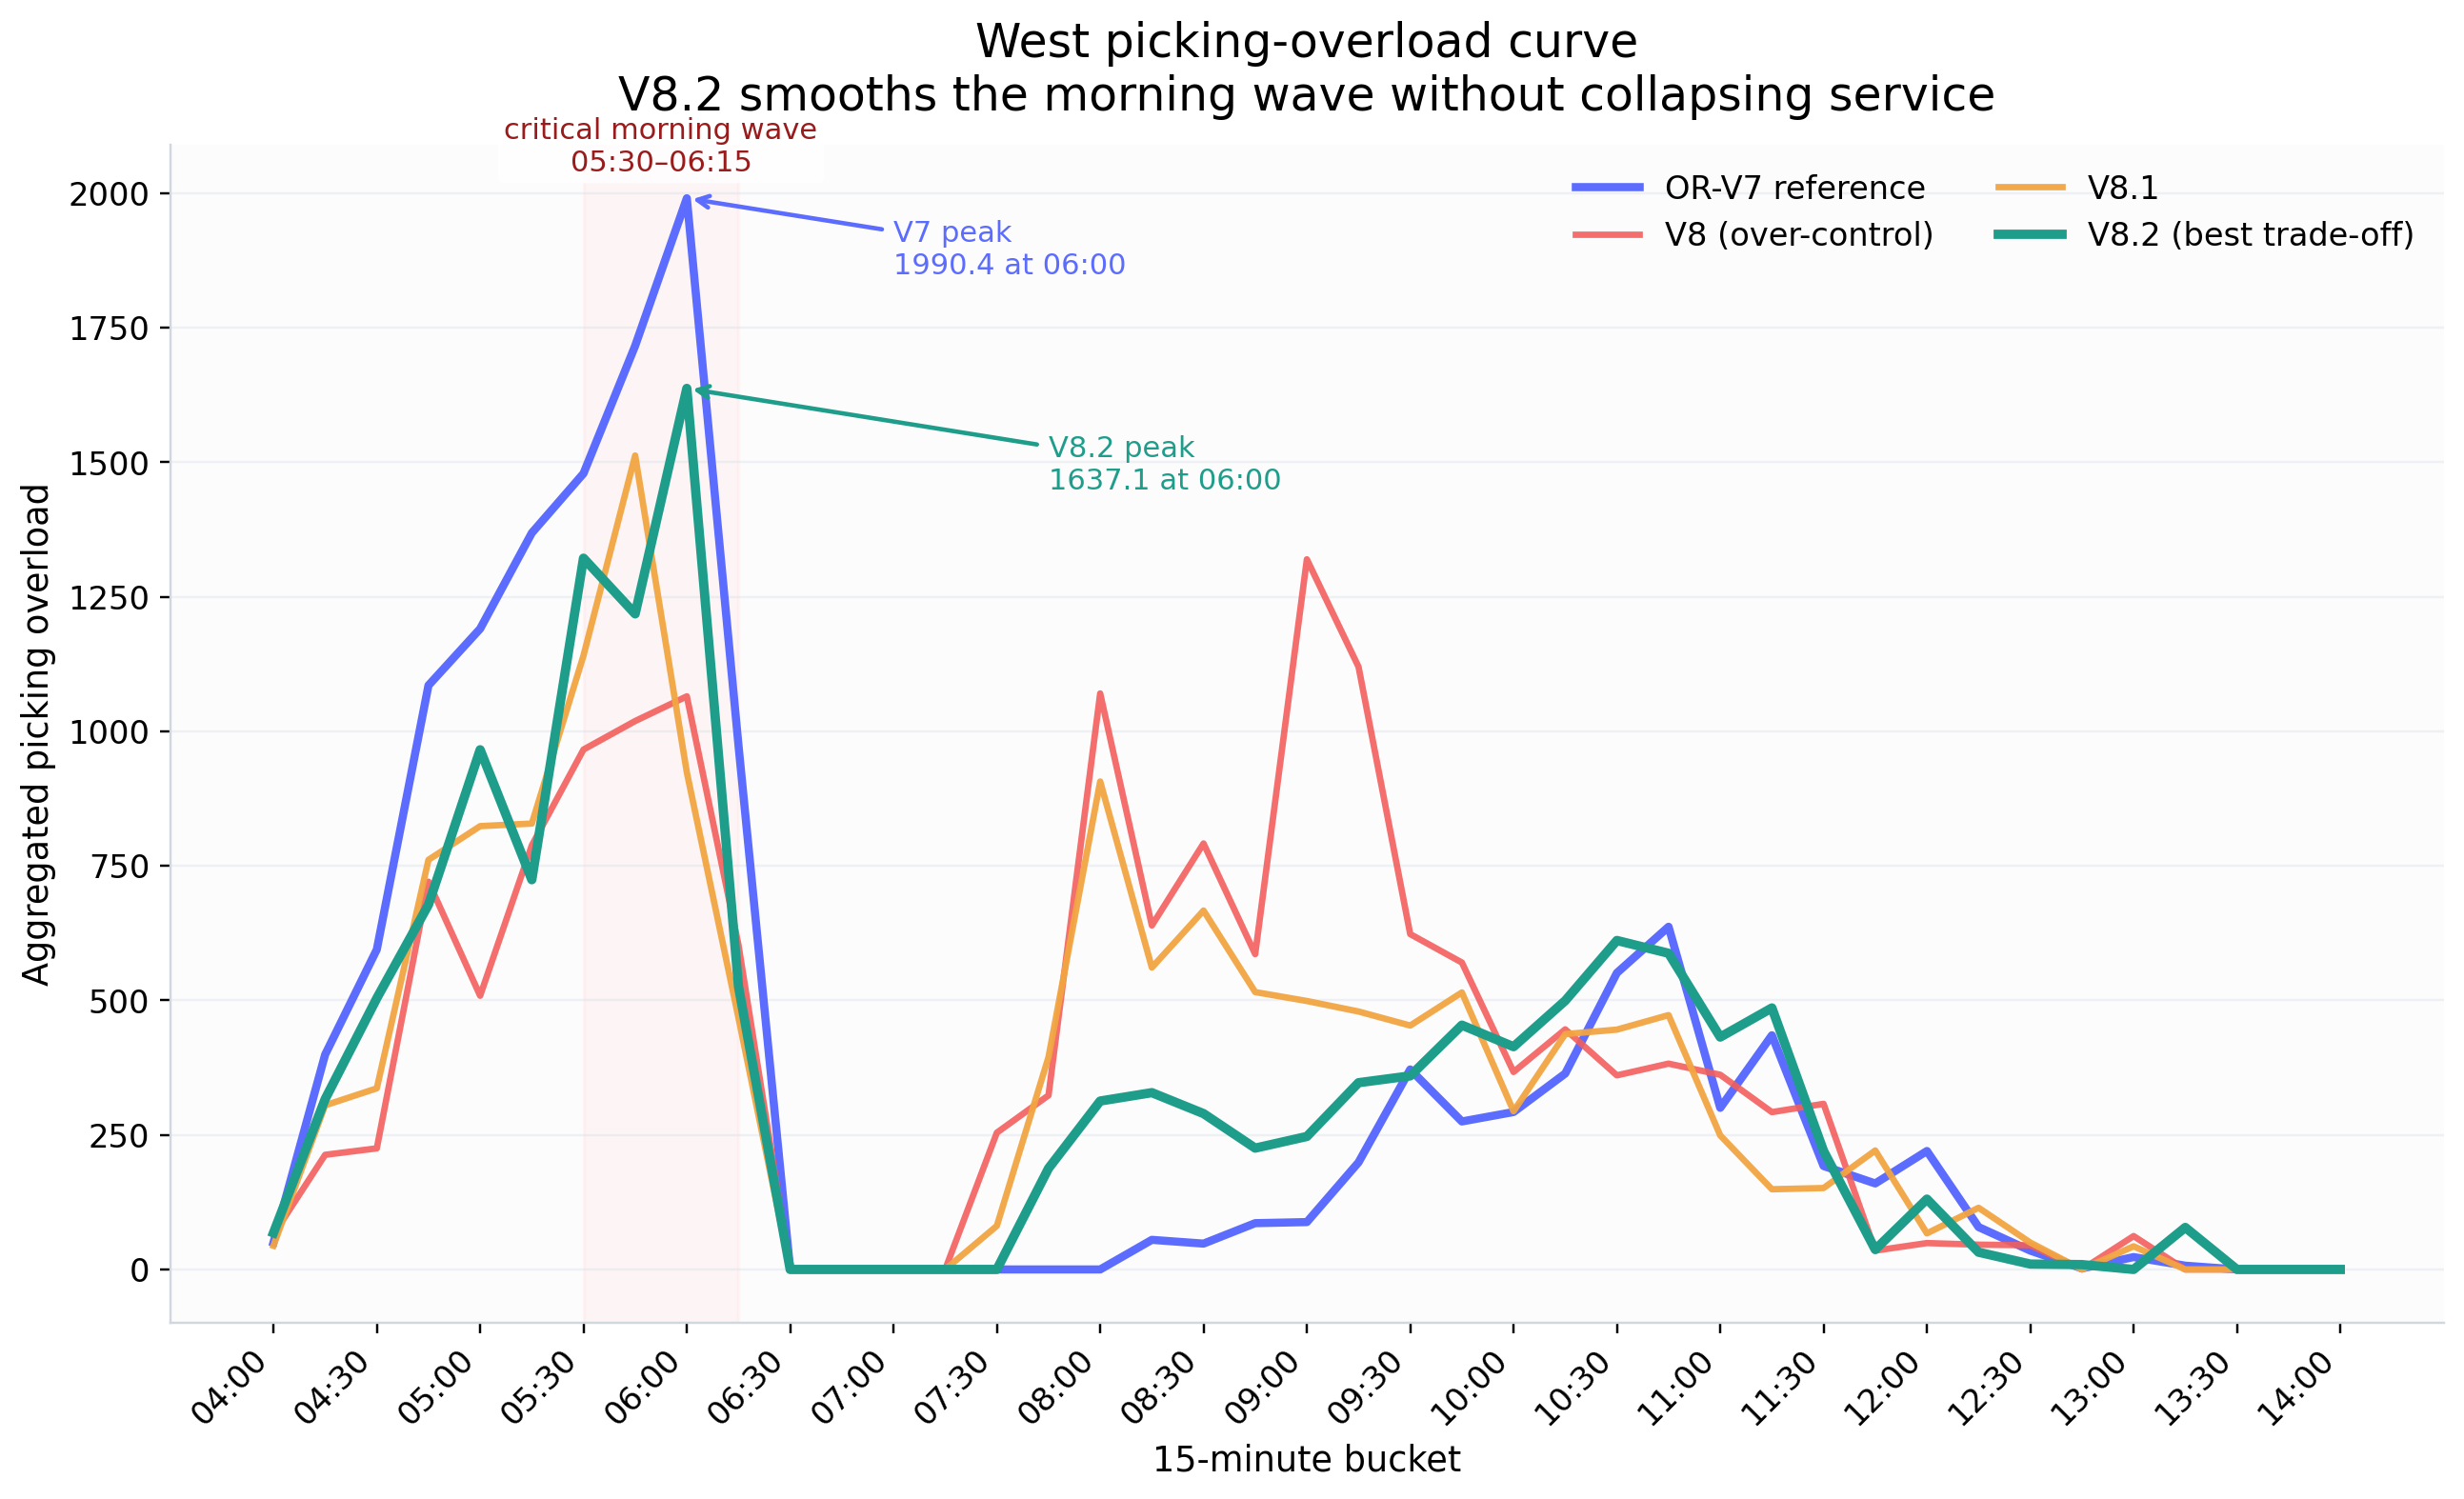
\includegraphics[width=0.98\textwidth]{Pictures/professor_preview/fig_west_picking_curve_comparison.png}
    \caption{Figure 7.1 compares West picking-overload curves across OR-V7, V8, V8.1, and V8.2. The critical 05:30--06:15 morning wave remains visible in all variants, but V8.2 lowers the dominant peak without the severe late-morning peak migration observed in the first V8 version.}
    \label{fig:west_picking_curve_comparison}
\end{figure}

This visual comparison is important for the thesis argument because it turns the smoothing claim into something operationally interpretable. The reader can see that the relevant improvement is a better service--smoothing trade-off, not simply a lower aggregate penalty number.

This is especially important because the earlier V8 versions show what failure looks like. The first V8 version dropped service to roughly 96.99\% and pushed overload into a later 08:00--09:00 peak, demonstrating that dynamic pricing can overreact. V8.1 recovered service to about 98.42\% and improved smoothing, but still created a stronger secondary wave than desired. V8.2 is the first version that both keeps service near the strong baseline regime and reduces the critical morning pressure without simply relocating it into a new late-morning bottleneck. For this reason, West is the clearest case in which the integrated controller-routing-repair line provides meaningful additional value beyond the earlier controller-centered reference line.

\section{Herlev and East: medium- and low-pressure regimes}

Herlev and East show that the value of the integrated dynamic-shadow-price mechanism is not uniform across instances. Herlev represents a medium-pressure regime in which depot sensitivity is still meaningful, but the system is not as extreme as West. East represents a looser regime in which the earlier OR-style baseline is already very strong.

On Herlev, V8.2 improves upon OR-V7 in a meaningful way. The integrated line increases delivered orders from 1035 to 1039 out of 1044 eligible orders, reduces deadline failures from 9 to 5, and lowers deferred events from 550 to 474. This is an important result because it shows that the smoothing logic is not useful only on the most extreme large-scale instance. Herlev still contains enough depot-side pressure for bucket-aware coordination to matter, and the resulting service improvement confirms that dynamic smoothing can help beyond the hardest stress regime.

East provides the corresponding boundary case. Under OR-V7, East already achieves 100\% within-window service. Under V8.2, delivered orders fall slightly from 3268 to 3259 out of 3268 eligible orders, corresponding to about 99.72\% service, while deadline failures rise from 0 to 9. Although some process metrics improve, the service loss is real. This shows that the V8.2 mechanism is not a universal improvement that should simply be activated at the same strength on every instance. On a relatively loose regime, strong bucket-aware smoothing can introduce unnecessary conservatism.

Taken together, Herlev and East support a regime-dependent interpretation. V8.2 is not only a West-specific trick, since it also helps on Herlev. But it is also not a globally dominant rule. Its value depends on whether the instance genuinely suffers from pressure patterns that are worth smoothing. This is one of the most important findings of the thesis, because it shifts the interpretation of dynamic shadow prices from ``best method'' to ``best mechanism under the right pressure regime.'' 

Table~\ref{tab:regime_summary} condenses this cross-instance story. It is included to help the reader quickly see that the same mechanism behaves differently across high-, medium-, and low-pressure settings.

\begin{table}[H]
    \centering
    \caption{Table 7.2 summarizes the three main integrated-solver regimes. West shows the clearest high-pressure gain from V8.2, Herlev also improves, while East demonstrates that dynamic smoothing is not universally dominant and should be activated with regime awareness.}
    \label{tab:regime_summary}
    \footnotesize
    \setlength{\tabcolsep}{4pt}
    \begin{tabularx}{\textwidth}{>{\bfseries\raggedright\arraybackslash}p{1.45cm} >{\centering\arraybackslash}p{1.35cm} >{\centering\arraybackslash}p{1.45cm} >{\centering\arraybackslash}p{1.45cm} >{\centering\arraybackslash}p{2.2cm} >{\centering\arraybackslash}p{2.45cm} >{\raggedright\arraybackslash}X}
        \toprule
        Instance & Regime & OR-V7 SR & V8.2 SR & Deadline failures & Morning picking over & Interpretation \\
        \midrule
        West   & High   & 99.93\%  & 99.41\% & 3 $\rightarrow$ 27 & 14901 $\rightarrow$ 13997 & Strong gain under high pressure \\
        Herlev & Medium & 99.14\%  & 99.52\% & 9 $\rightarrow$ 5  & --- & Moderate service gain \\
        East   & Low    & 100.00\% & 99.72\% & 0 $\rightarrow$ 9  & --- & No free win in a loose regime \\
        \bottomrule
    \end{tabularx}
\end{table}

The summary table also reinforces the thesis claim that dynamic shadow pricing should be interpreted as regime-sensitive coordination rather than as a universal drop-in improvement. That point becomes important again when the thesis compares the retained controller-centered line with the newer integrated solver line.

\section{Cross-system comparison through aligned top-level KPIs}

The retained controller-centered line and the integrated solver line should not be flattened into a single best-model ranking table, because they are not identical systems with identical internal semantics. Their routing backends, depot representations, and process metrics differ. However, the two lines can still be compared safely through the aligned paper-facing KPI schema introduced in Chapter~\ref{chap:experimental_design}.

Under that aligned schema, both lines can report eligible orders, delivered orders within window, deadline failures, and the resulting within-window service rate. This makes it possible to compare high-level service outcomes without pretending that all internal process quantities are directly commensurate. In this sense, the retained controller line remains the mature controller-centered reference language, while the integrated line provides a richer architecture-level and depot-aware interpretation.

The safe conclusion is therefore not that the integrated line has simply replaced the retained line. Rather, the thesis now contains two layers of evidence. The retained line shows that rolling-horizon admission control can be improved in a disciplined, paper-facing progression. The integrated line shows that some remaining failures are more naturally resolved when depot-wave pressure is internalized more explicitly into the solving architecture. This is a readable and defensible comparison. It is not a claim that both systems are interchangeable solver versions.

\section{Computational efficiency and implementation trade-offs}

The two method lines also differ in implementation style and computational profile. The retained controller-centered line is rooted in a more established Python-based experiment workflow in which the controller is the primary research object and the daily routing backend is used as a supporting execution layer. This line is especially strong in experiment discipline, seed-based benchmarking, and paper-facing result management.

The integrated line, by contrast, benefits from a Julia-first implementation that is more naturally suited to repeated large-scale constructive search, matrix-based feasibility checks, and depot-aware route evaluation. This does not imply that implementation language alone explains the quality difference. Rather, the computational trade-off is architectural. The integrated solver performs more work inside the route-construction and repair loop, which would be awkward to study if the whole contribution remained at the controller layer only.

From a practical thesis perspective, the two lines therefore offer different advantages. The retained line offers the clearer paper-facing progression and the cleaner controller-centered comparison chain. The integrated line offers stronger architectural realism and richer diagnostics, especially on the largest and most wave-sensitive instances. Their coexistence in the thesis is not a weakness. It reflects the fact that understanding this warehouse-distribution problem requires both a strong rolling-horizon admission reference and a more explicit depot-aware solving perspective.
